\documentclass{strategynet-journal}
\hypersetup{pdftitle={Jörmungandr: Adapting a Language Model to Tool Use},pdfauthor={research@strategynet.ai}}
\SNHeader{strategynet.ai:Jormungandr}
\title{Jörmungandr: Adapting a Language Model to Tool Use}
\author{\href{mailto:research@strategynet.ai}{research@strategynet.ai}}
\date{November 2026}
\begin{document}
\maketitle
\begin{abstract}
A language model given access to tools must choose which one to use and respond
to evidence about whether it worked. We apply Jörmungandr's learning framework
to that decision: a small pretrained language model scores available services
from their descriptions and its recent verified call history. Training uses
the outcomes of chosen calls. During evaluation the weights remain fixed,
while new observations update the history supplied to the model.

Two independently trained policies met a predefined comparison against simple
history-based rules across seven reserved tasks. The largest shortfall was
2.002 percentage points. This establishes tool selection for known jobs under
the tested changes in reliability; it does not establish general API discovery,
better free-form answers, or an advantage over simpler methods.

Separate numeric studies examine mechanisms that could support later
language-model work: extra context objectives, delayed rewards, and preference
feedback. The extra objectives brought little benefit to decisions. Longer
returns improved early learning when rewards were delayed, and explicit
comparisons recovered simulated preferences more reliably than biased clicks.
These supporting results have not yet been demonstrated in a language model.
\end{abstract}
\SNtwocolumntableofcontents

\section{From learning trading decisions to choosing tools}
\begin{SNcolumns}

Jörmungandr was developed to separate a learning algorithm from the application
that supplies observations, actions, and rewards. In a trading application,
those actions may be holding, closing, or changing an exposure. In the present
application, the action is a tool call and its immediate outcome can be checked
by a verifier. The surrounding learning problem changes, while the need to
preserve decision-time information and evaluate independently remains.

The companion paper, \href{https://strategynet.ai/white-papers/jormungandr-plugin-runtime.pdf}{\emph{A Plugin Runtime for Distributed Reinforcement Learning}},
explains the algorithms, infrastructure, structured actions, and financial
application interfaces. This paper concerns the new language-model work:
what we trained, how we tested it, and which further mechanisms are promising
enough to investigate.

A pretrained language model already contains useful representations of text,
but it cannot know that a particular service has recently become unreliable
unless that evidence reaches its input. Nor does a plausible tool choice
establish that the tool produced a correct result. We therefore separate
three responsibilities: the model chooses, the service executes, and an
independent check supplies the outcome used for learning.

\subsection{Related work}

LoRA provides a way to adapt a pretrained model by learning compact low-rank
weight changes while leaving the original weights fixed~\cite{lora}. It
reduces the number of parameters that must be trained; the task and learning
objective still have to be specified. We use it to adapt a small model to
score candidate tools from recent evidence.

ContextRL studies a related information problem: whether a language model can
identify the part of its context that supports an answer~\cite{contextrl}.
Its additional objective asks the model to choose between similar contexts.
This motivated a separate numeric experiment in our work. That experiment
uses different tasks and learning methods and does not reproduce ContextRL's
language-model results.

Feedback also need not be an automatically verified success or failure.
Christiano and colleagues showed how comparisons between behavior sequences
can supply a learned objective~\cite{preferences}. We investigate the narrower
question of ranking several acceptable options from explicit preferences or
clicks. The distinction between those feedback sources matters before they
are used to train any language model.

\section{The tool-selection task}

\subsection{What the model observes}

Several services accept the same known type of job. Their reliability can be
stable, change during a session, or include random failures. The model must
choose a service using only evidence available before the call.

Its input contains the request, available services, and its own sixteen most
recent calls. Counts, recency, and outcome summaries are derived from that
same history. The model sees the verified result of the service it selected;
it does not see the results of unchosen services, the hidden reliability
parameters, or the time at which reliability changes.

This makes history informative without giving the model the answer. Service
names and request wording change during evaluation, and candidate order is
shuffled. These checks make it harder to succeed by memorizing an identifier
or a row position instead of using the recorded evidence.

\subsection{What is trained}

We adapt SmolLM2-135M~\cite{smollm2} with LoRA and a head that assigns a reward
score to each candidate. The target is the verified outcome of the chosen
call. With the future-reward discount set to zero, the score learns expected
immediate reward from the current context. Although implemented through a
value-learning interface, this experiment is a contextual bandit problem:
it does not train a long-horizon planner or a token-by-token answer generator.

Collection initially mixes random choices with a rule based on recent success
rates. Subsequent refinement also uses histories encountered by the learned
policy. This matters because a policy changes the observations it collects:
a model trained only on another policy's histories may encounter unfamiliar
situations when it makes its own choices.

Every evaluated policy, including the statistical references, uses the same
10\% random exploration rule. Exploration costs are included in its reward.
The model is learning a score for choosing among tools; it is not learning
when or how much to explore.

\subsection{Adaptation during a session}

There are two different ways a system can adapt. Training changes its weights.
A new observation can also change its decision without any weight update,
provided that observation appears in the next input. Our evaluation tests the
second form: weights are frozen, but the history changes after each call.

For example, a service that has worked repeatedly may fail. The next decision
can use that failure together with older outcomes. One failure is not proof
that a service is permanently unreliable, especially in the noisy tasks.
The task tests how the learned score uses accumulated evidence, rather than
whether the model can be retrained after every response.

\end{SNcolumns}
\section{Results of the language-model experiment}

Two independently trained models were frozen before confirmation. Each was
assessed on seven reserved tasks, with 32 simulated worlds per task and 128
calls per world. The comparison therefore contains 57,344 model decisions,
but only two independent training runs. The number of calls should not be
mistaken for a large sample of independently trained models.

Each model was compared with rules based on the last outcome, recent mean
success, and a recent-mean score with an exploration bonus. The policies faced
matched underlying service outcomes but maintained their own histories. The
predefined acceptance rule allowed at most a five-percentage-point shortfall
from the strongest reference on any task, plus minimum performance on stable
tasks.

\begin{table}[H]
\centering
\small
\caption{Mean verified reward on reserved tasks. Each reference column gives
the strongest matched rule for that task and training run. Values are rounded
to three decimals; the unrounded largest shortfall was 0.02002.}
\begin{tabular}{lrrrr}
\toprule
& \multicolumn{2}{c}{Training run 1} & \multicolumn{2}{c}{Training run 2} \\
Task & Language model & Reference & Language model & Reference \\
\midrule
Four services, stable & .913 & .913 & .916 & .916 \\
Eight services, stable & .882 & .882 & .885 & .885 \\
Four services, changing & .807 & .810 & .814 & .787 \\
Eight services, changing & .763 & .775 & .780 & .789 \\
Four services, noisy & .547 & .552 & .609 & .559 \\
Eight services, noisy & .497 & .515 & .530 & .508 \\
Eight services, harder & .440 & .456 & .439 & .459 \\
\bottomrule
\end{tabular}
\label{tab:language-results}
\end{table}

Both models met the acceptance rule. Neither consistently outperformed the
simpler references. Low rewards in noisy tasks partly reflect unreliable
services and the common exploration rule; a value near 0.5 is not a binary
classification accuracy. Checks also confirmed that the exported models
preserved candidate-order behavior and made executable HTTP calls with
verified results.

\begin{SNcolumns}
\subsection{What changed after the earlier failures}

The passing result followed unsuccessful training attempts. Using histories
visited by the learned policy, together with explicit counts and recency,
improved the final setup. These changes were introduced together, so the
experiment cannot assign the gain to either change alone. No weights from
a separately trained numeric policy were transferred into the language model.

Removing all history in balanced controls reduced performance to the random
selection rates of 25\% for four services and 12.5\% for eight. That supports
the role of recent evidence in this task. It does not establish that the
language-model representation is necessary: the statistical references also
use history and remain strong alternatives.

\subsection{What this result means}

We have a language policy that can use recent verified outcomes to choose
among known services under the tested conditions. It can be trained and
executed through the same framework used for other decision problems.

The experiment does not show that a model has learned arbitrary API semantics,
improved the factual quality of its prose, or learned a financial strategy.
The job type was supplied, the services were defined in advance, and an
independent verifier was available. The next evaluation needs new reserved
tasks because these confirmation results have already informed development.

\section{Supporting studies for future language-model work}

The following studies use small numeric models rather than language models.
They test individual mechanisms cheaply enough to compare several controls.
Their relevance to the language application is a reason to test them there,
not evidence that they have already improved it.

\subsection{Does an extra context objective improve decisions?}

Supplying history solved an information problem in tool selection. We next
asked whether an additional objective could teach a model to use that history
more effectively. The context-selection task required distinguishing two
histories that differed in the order of outcomes while preserving their
counts. This prevented success from simple counting alone.

We compared reward-only learning with context selection, direct factual
supervision, and additional reward-only updates. The extra objectives learned
their tasks, but did not improve final average reward. Separate noisy-state
experiments asked models to forecast observations and identify observable
changes. Those objectives also learned, while final reward gains remained
about 0.02--0.06 percentage points with no sustained early-learning advantage.

The practical lesson is to measure the decisions an auxiliary task improves,
not just its own prediction accuracy. These results do not justify making
such objectives a default. They also do not refute ContextRL: the models,
tasks, and training procedure differ.

\subsection{When the outcome arrives later}

Tool success in the confirmed experiment is checked immediately. A longer
workflow may return a useful outcome only after several choices. The learner
must then connect that outcome to earlier actions.

A one-step value target passes information backward through successive
updates. A multi-step return includes several observed rewards in the same
target. It can carry a delayed outcome back sooner, but may have greater
variance and, when intermediate actions come from another policy, bias.
Generalized Advantage Estimation develops a related tradeoff over reward
horizons for policy-gradient methods~\cite{gae}.

We isolated delay with one meaningful choice followed by forced waits. After
128 updates with a twelve-step reward delay, initial-choice accuracy was
85.9\% for one-step learning and about 94\% for four- and thirteen-step returns.
All methods used the same recorded episodes. Immediate rewards favored
one-step learning early, and final performance after 512 updates was similar.
The finding concerns earlier learning under delay, not a higher final accuracy
or a demonstrated improvement to a language model.
\end{SNcolumns}

\begin{figure}[H]
\centering
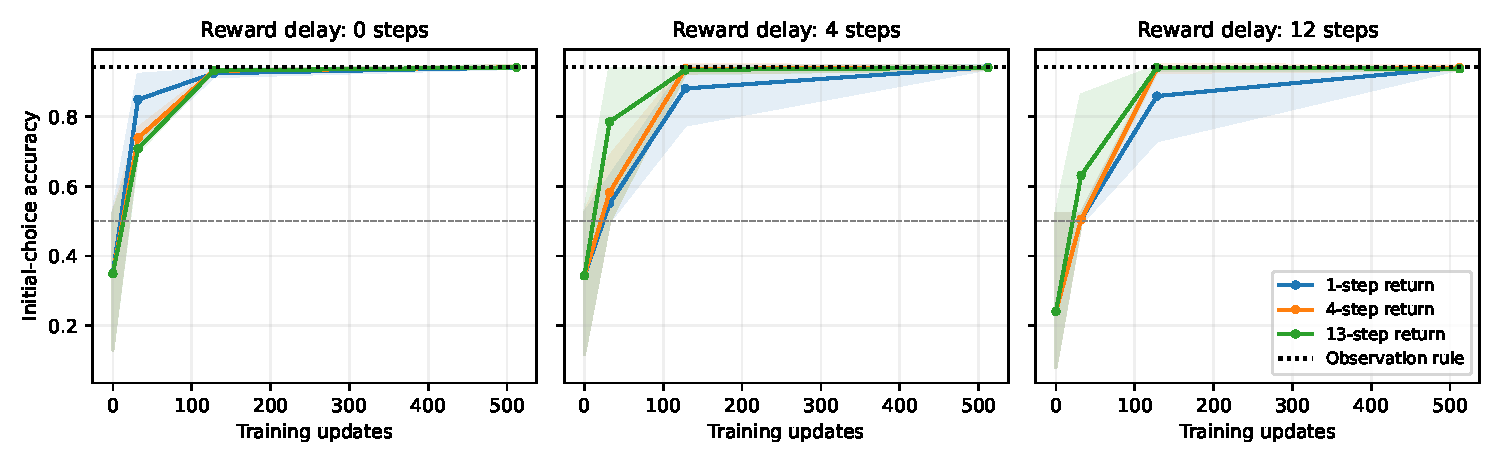
\includegraphics[width=.96\textwidth]{figures/delayed_credit_learning.pdf}
\caption{Opening-choice accuracy with immediate and delayed rewards. Curves
average four noise and reward-frequency conditions. Shading is the range
across three training runs, not a confidence interval. The dotted line is a
fixed rule using the observed cue; the dashed line is random choice.}
\end{figure}
\begin{SNcolumns}

A response delayed by a network is a separate issue. Its outcome still belongs
to the original action, not whichever action is current when it arrives.
The application must match those records before presenting finalized
experience to the learner. An unknown outcome cannot be treated as a failed
call or a zero reward without changing the meaning of the data.

\subsection{Several answers may be useful}

A user may prefer one answer even when several are acceptable. Preference
learning addresses that relative judgment; it does not necessarily label an
answer correct or incorrect. Our study records what was displayed and its
order separately from the feedback that followed.

An explicit comparison says which of two candidates is preferred. A click
also depends on whether the user noticed the alternatives and where they
appeared. Treating every unselected answer as inferior can therefore teach
the scorer a display-position bias.

In a six-option simulation, three options were acceptable under a known
utility function. After 1,024 feedback events and 512 training updates,
explicit comparisons recovered 97.0\% of the acceptable options in the top
three. Biased clicks recovered 57.2\%; randomizing display order raised this
to 75.4\%. The simulated users were deliberately position-biased. These
percentages are not measurements of real users, and explicit comparisons
require different human effort from clicks.
\end{SNcolumns}

\begin{figure}[H]
\centering
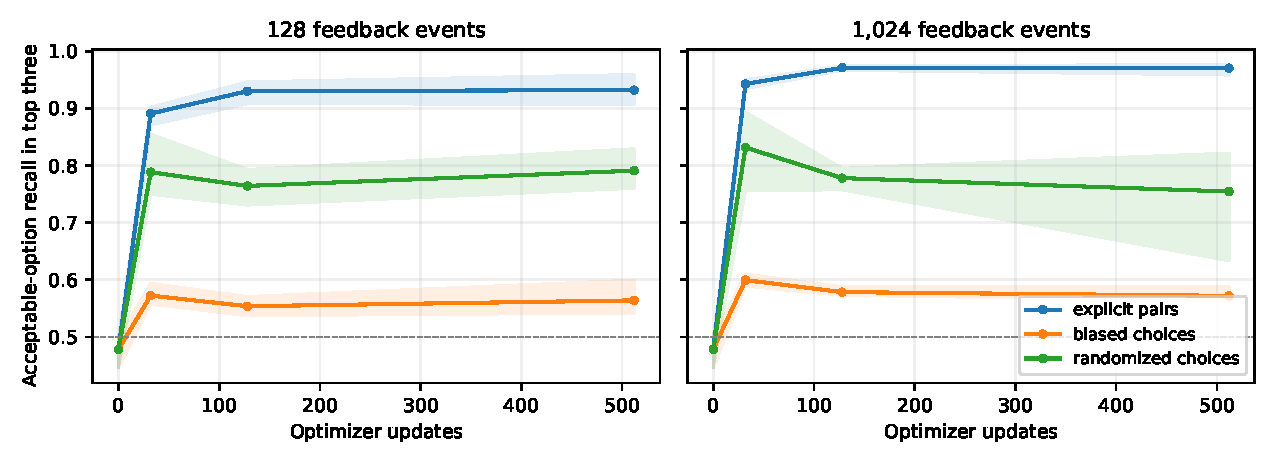
\includegraphics[width=.88\textwidth]{figures/shortlist_preference_learning.pdf}
\caption{Recovering three acceptable options in a six-option simulation.
Bands show the range across three training runs. Random ranking has expected
recall 0.5. These experiments compare feedback assumptions, not annotation cost.}
\end{figure}
\begin{SNcolumns}

This supplies a tested preference-learning component, not a completed
language-model feedback loop. No LLM was trained in this study, and real-user
collection requires its own evaluation. Recording queries or clicks alone
does not automatically improve a model.

\section{What we have established and what comes next}

The completed language-model result is tool selection from recent verified
history. It uses actual outcomes for training and remains close to strong
simple references on the reserved tasks. The supporting studies identify
options for later work: multi-step rewards merit investigation for longer
workflows, while preference comparisons require a deliberate collection
policy. The tested auxiliary objectives have not earned their additional cost.

A next study should compare the language policy and simpler rules on fresh
tool-selection problems, report inference and training cost, and vary model
size and adaptation method. Longer workflows need several consequential
actions before reward, rather than forced waits. Preference work needs real
judgments and an evaluation of whether those judgments improve useful answers.
Those are separate claims and should be tested separately.

\section*{Research materials}
The \href{https://github.com/ingvor-restrat/jormungandr/blob/main/docs/multiservice_adaptation.md}{tool-selection report}
contains the earlier failures, training controls, and reserved comparison.
The \href{https://github.com/ingvor-restrat/jormungandr/blob/main/docs/context_auxiliary_research.md}{context-objective study},
\href{https://github.com/ingvor-restrat/jormungandr/blob/main/docs/noisy_state_auxiliary.md}{noisy-observation study},
\href{https://github.com/ingvor-restrat/jormungandr/blob/main/docs/delayed_credit.md}{delayed-reward study}, and
\href{https://github.com/ingvor-restrat/jormungandr/blob/main/docs/shortlist_preferences.md}{preference study}
provide their protocols and recorded results. Figures here are regenerated
from those results; no model was retrained for this paper.
\end{SNcolumns}

\begin{thebibliography}{99}

\bibitem{gae}
J. Schulman, P. Moritz, S. Levine, M. Jordan, and P. Abbeel,
\emph{High-Dimensional Continuous Control Using Generalized Advantage
Estimation},
International Conference on Learning Representations, 2016,
\url{https://arxiv.org/abs/1506.02438}.

\bibitem{lora}
E. J. Hu et al.,
\emph{LoRA: Low-Rank Adaptation of Large Language Models}, 2021,
\url{https://arxiv.org/abs/2106.09685}.

\bibitem{smollm2}
Hugging Face,
\emph{SmolLM2-135M model card},
\url{https://huggingface.co/HuggingFaceTB/SmolLM2-135M}.

\bibitem{contextrl}
P. Xu et al.,
\emph{Context-Aware RL for Agentic and Multimodal LLMs},
arXiv:2606.17053v1, June 2026,
\url{https://arxiv.org/abs/2606.17053v1}.

\bibitem{preferences}
P. Christiano, J. Leike, T. B. Brown, M. Martic, S. Legg, and D. Amodei,
\emph{Deep Reinforcement Learning from Human Preferences},
Advances in Neural Information Processing Systems, 2017,
\url{https://arxiv.org/abs/1706.03741}.



\end{thebibliography}
\end{document}
